\section{System's Perspective}

\subsection{Design and Architecture}
Figure \ref{fig:systemoverview} provides an overview of our system infrastructure:
\begin{figure}[H]
    \centering
    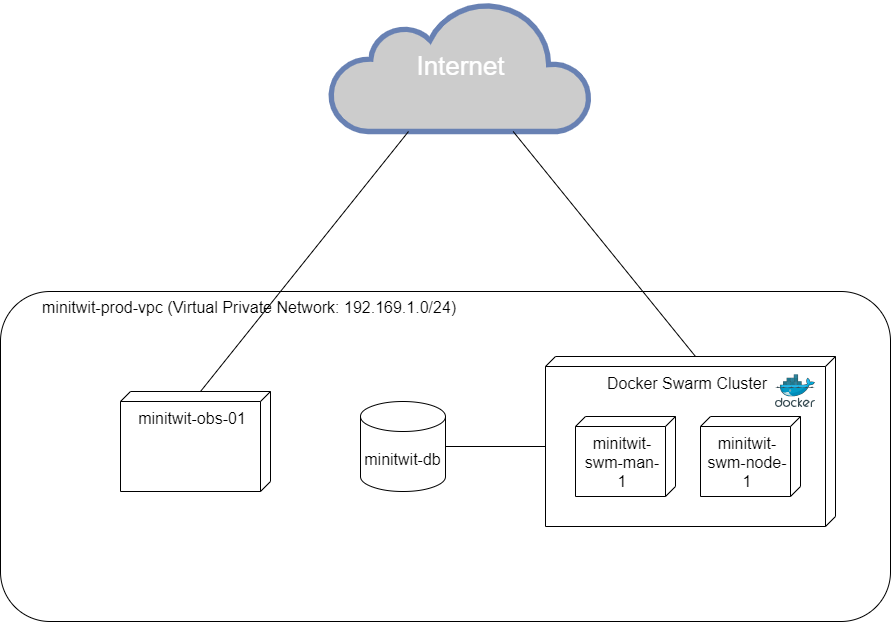
\includegraphics[width=0.7\linewidth]{images/system-overview3.png}
    \caption{Overview of the system infrastructure}
    \label{fig:systemoverview}

\end{figure}
The system includes a single Virtual Private Network with an IP range 192.168.1.0/24. Within this network, we operate a database cluster consisting of a single node. This node is connected to the Docker Swarm cluster, featuring a manager and a worker node.

Both our monitoring and cluster servers are visibly exposed to the internet. Additionally, the database server is accessible from the internet, but has a constraint of only talking to our servers and therefore not accepting requests from other hosts.

\subsection{Interactions of Subsystems}
Our system consists of two main subsystems, namely the REST SimulatorAPI and the webapplication Minitwit. As seen in Figure \ref{fig:subsystem-interaction}, the SimulatorAPI and Minitwit subsystems are similar in structure. However, when looking at the processes behind the structures in Figure \ref{fig:frontend-interaction} and \ref{fig:backend-interaction}, it is apparent that these two differ greatly.

\begin{figure}[H]
    \begin{center}
        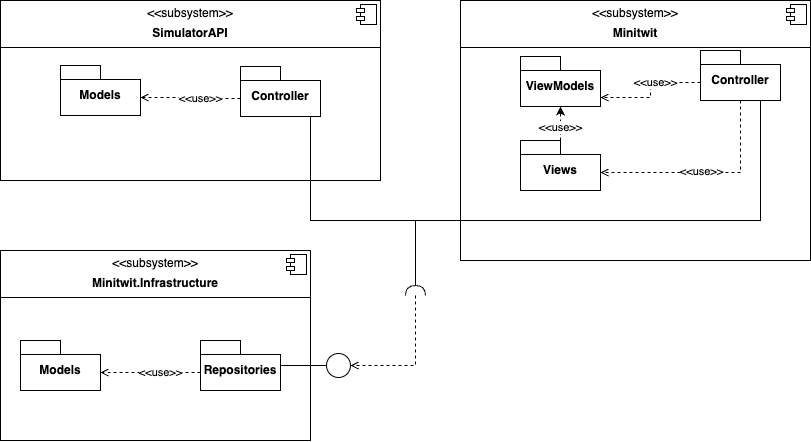
\includegraphics[width=1\textwidth]{Subsystem-Interaction.png}
    \end{center}
    \caption{An overview of the subsystems and how they interact}
    \label{fig:subsystem-interaction}
\end{figure}

Because the two main subsystems are inherently different, we wanted to implement a database abstraction layer such that we had a uniform way of querying the database. Therefore, both controllers use the Repository package from the subsystem Minitwit.Infrastructure to query the database using the Repository pattern\cite{repo_pattern}.
%cite
Due to the different specifications for Minitwit and SimulatorAPI, the controller for Minitwit is more complex. As seen in Figure \ref{fig:frontend-interaction}, the controller for Minitwit has to present information in a GUI, whereas the SimulatorAPI only calls the repository to fetch the user messages, as seen in Figure \ref{fig:backend-interaction}.
\begin{figure}[H]
    \begin{center}
        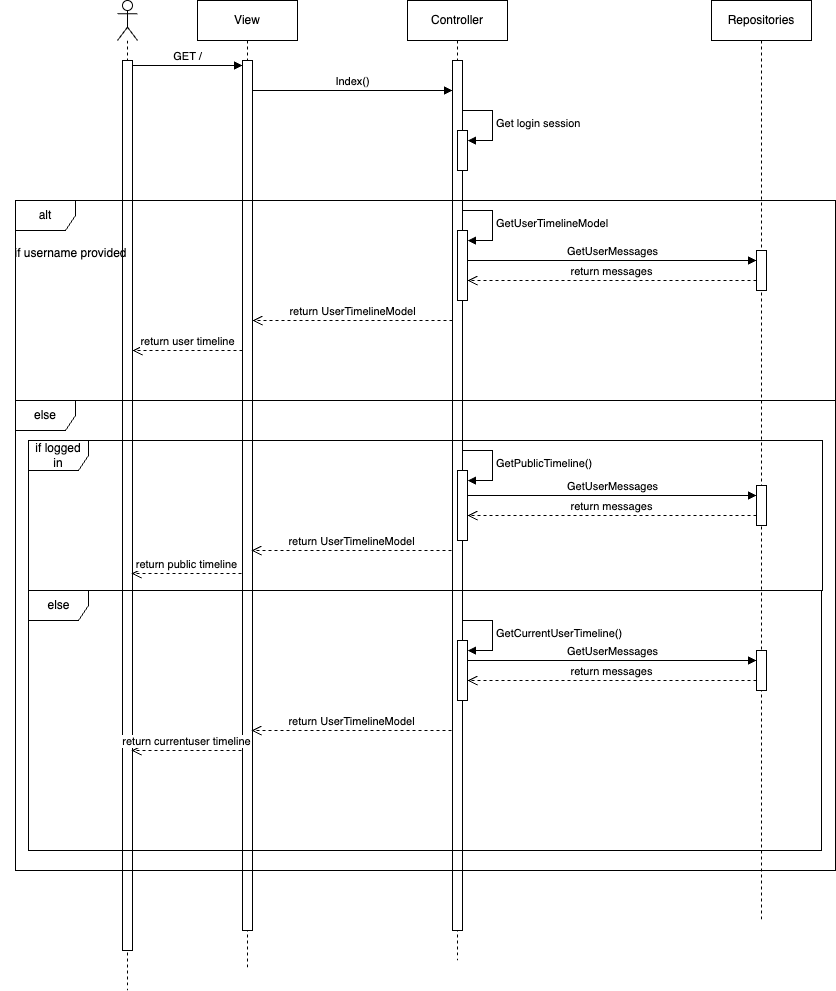
\includegraphics[width=1\textwidth]{Fronted-Sequence-Diagram.png}
    \end{center}
    \caption{Minitwit: Sequence diagram of a user call to the index page}
    \label{fig:frontend-interaction}
\end{figure}
\begin{figure}[H]
    \begin{center}
        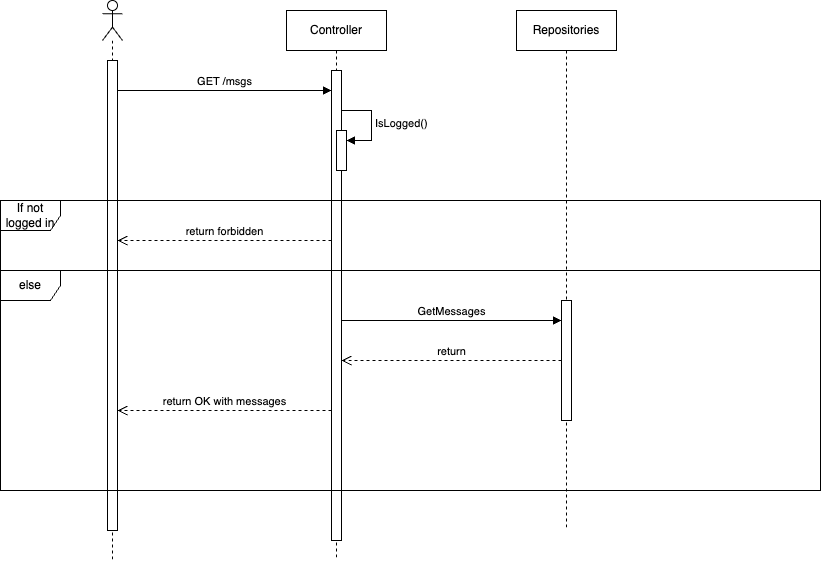
\includegraphics[width=1\textwidth]{Backend-Sequence-Diagram.png}
    \end{center}
    \caption{SimulatorAPI: Sequence diagram of a user call to get messages}
    \label{fig:backend-interaction}
\end{figure}


\subsection{Dependencies, Technologies and Tools}

% All dependencies of your *ITU-MiniTwit* systems on all levels of abstraction and development stages. That is, list and briefly describe all technologies and tools you applied and depend on.

In Table \ref{tab:tool} we briefly describe the tools and technologies used. A comprehensive list of tools containing the full reasoning for their use, can be found in appendix \ref{appendix:decision-log}.

\begin{longtable}{|p{0.3\textwidth}|p{0.2\textwidth} | p{0.4\textwidth}|}
    \hline
    \textbf{Purpose} & \textbf{Technology/Tool} & \textbf{Description}\\
    \hline
    Work log & \href{https://www.notion.so/help/guides/category/documentation}{Notion} & Notion is a web hosted workspace, that allows users to collaborate in real-time on managing projects, notes, and other types of documents in a markdown format.\\
    \hline
    Remote Repository, work tracking, and coordination & \href{https://github.com/features}{GitHub} & GitHub serves as a remote Git repository. It comes with collaborative features, such as having work items (known as issues), project coordination boards, CI/CD workflows, etc. We use GitHub, as the group has experience with the tool and it provides the collaborative features we need.\\
    \hline
    Programming language & \href{https://learn.microsoft.com/en-us/dotnet/csharp/}{C\#} &
    C\# is an object-oriented programming (OOP) language. We chose C\# due to its widespread use in the industry, making it very well documented. Furthermore, the familiarity of OOP paradigms among developers served as a supplementary factor.\\
    \hline
    Micro Web-Framework & \href{https://learn.microsoft.com/en-us/aspnet/core/razor-pages/?view=aspnetcore-8.0&tabs=visual-studio}{Razor Pages} & Razor Pages is a simple web application programming model provided by ASP.NET. It uses C\# and simple markup syntax in order to build web pages. Furthermore, Razor Pages offers simple configuration and an abundance of documentation.\\
    \hline
    Database Connection & \href{https://learn.microsoft.com/en-us/ef/core/}{Entity Framework} & Entity Framework (EF) serves as an object-relational mapper, which allows developers to work with databases using .NET objects. It also eliminates the need for data-access code, by using LINQ in order to interact with the data.\\
    \hline
    Server host & \href{https://docs.digitalocean.com/}{Digital Ocean} & Digital Ocean (DO) is a cloud hosting service, which provides server hosting, database hosting, and a command line interface tool (doctl), that can be used to automatically create and drop droplets (VMs). We have chosen DO primarily due to the great documentation and online resources.\\
    \hline
    Database & \href{https://www.postgresql.org/docs/}{PostgreSQL} & PostgreSQL is an open source relational database management system known for its extensibility, and adherence to SQL standards. Additionally, the majority of developers in the team have previous experience with PostgreSQL.\\
    \hline
    CI/CD & \href{https://docs.github.com/en/actions}{GitHub Actions} & GitHub Actions is a CI/CD service, that allows the user to automate tasks such as building, testing, and deploying code when certain conditions are met. GitHub Actions is well documented, and it is quite seamless to configure secrets and refer to them in a \texttt{.yaml} file. Due to its integration with GitHub, we chose GitHub Actions, as we already use GitHub to store our code repository. Furthermore, it collaborates well with other tools used in the project, such as Digital Ocean.\\
    \hline
    Monitoring and Logging Graphics & \href{https://grafana.com/}{Grafana} & Grafana is a well known open source monitoring toolbox, that includes a variety of features such as visualising monitoring metrics and logging via customisable dashboards.\\
    \hline
    Metrics collector & \href{https://prometheus.io/docs/}{Prometheus} & Prometheus is a monitoring and alerting toolkit, that scrapes and stores data from a specific application, alerting developers of abnormalities in the system. The only requirement we had for a metrics collector was: It had to collaborate with Grafana.\\
    \hline
    Metrics collector & \href{https://opentelemetry.io/docs/languages/}{OpenTelemetry} & OpenTelemetry is a metrics collector, that supports a variety of different APIs and SDKs such as .NET. We chose OpenTelemetry since it is widely used, and it is well integrated with .NET applications.\\
    \hline
    Quality of Code Analysis & \href{https://www.sonarsource.com/products/sonarcloud/}{SonarCloud} & SonarCloud is a cloud based code analysis service, which can be integrated into a GitHub repository, in order to analyse the code in said repository.\\
    \hline
    Linter & \href{https://pre-commit.com/}{Pre-commit} & Pre-commit is a framework for managing pre-commit hooks. This can be used for automatically fixing code formatting and removing debug statements. We chose this tool as multiple actions can be integrated into one hook, as we were tasked with integrating three linters into the system.\\
    \hline
    Linter & \href{https://github.com/hadolint/hadolint}{Hadolint} & Hadolint is an open source Dockerfile linter, that enforces best practices when building Docker images. We have quite a few Dockerfiles, therefore we found it fitting to have a Dockerfile linter. Hadolint seems to be the more popular one as it is Haskell-based.\\
    \hline
    Formatter & \href{https://learn.microsoft.com/en-us/dotnet/core/tools/dotnet-format}{Dotnet-format} & Dotnet-format is a formatting tool, included in the .NET 6 SDK and onwards. It applies style preferences to a project which can be configured in an \texttt{.editorconfig} file. We chose dotnet-format since this linter enforces C\# coding conventions.\\
    \hline
    Logging & \href{https://grafana.com/docs/loki/latest/}{Grafana Loki} & Loki is a log aggregation system designed to store and query logs from an application, inspired by Prometheus. In order to implement a logging stack, we were interested in using a tool that was compatible with Grafana. Loki ensures this compatibility, as it is from the Grafana toolbox.\\
    \hline
    Infrastructure as code & \href{https://www.pulumi.com/docs/}{Pulumi} & Pulumi is an open source infrastructure as code SDK, that enables creation, deployment and management of infrastructure for a cloud service. We picked Pulumi, as it does not introduce a new programming language, it is open source, and it works well with CI/CD tools.\\
    \hline
    Configuration management & \href{https://docs.ansible.com/}{Ansible} & Ansible is an open source automation software used to configure and deploy systems using Ansible playbooks written in \texttt{.yaml} files. We chose Ansible as it provides an easy setup and does not require a new client to be installed on our application servers. Furthermore, the configurations is described in YAML, thereby not introducing new languages.\\
    \hline
    Scaling & \href{https://docs.docker.com/reference/cli/docker/swarm/}{Docker Swarm} & Docker Swarm is a container orchestration tool used for clustering Docker containers. Due to the team's limited experience with managing scaled systems, we chose Docker Swarm since we were already using Docker.\\
    \hline
    \caption{Tools and dependencies used in Minitwit}
    \label{tab:tool}
\end{longtable}


\subsection{Current State}
Table \ref{current-table} describes the status of the system after the simulator has ended.
\begin{table}[H]
    \begin{center}
        \begin{tabular}{ |c|c| }
            \hline
            Total requests & 34233 \\
            \hline
            Requests secured & 34233 \\
            \hline
            Total unhandled exceptions & 18 \\
            \hline
            P99 min response time & 94.2 ms \\
            \hline
            P99 max response time & 716 ms \\
            \hline
            Number of users &  116995\\
            \hline
            Avg followers per user &  28.5\\
            \hline
        \end{tabular}
    \end{center}
    \caption{System metrics}
    \label{current-table}
\end{table}
Furthermore, the static analysis tool SonarCloud assesses that the quality of the overall code is good (see appendix \ref{appendix:sonarcloud}).
